\documentclass[UTF8]{ctexbeamer}	% Compile at least twice!
%\setbeamertemplate{navigation symbols}{}
\usetheme{Antibes}
\usecolortheme{beaver}
\setbeamertemplate{navigation symbols}{}
% \useinnertheme{rectangles}
% \useoutertheme{infolines}
% \useoutertheme[title,section,subsection=true]{smoothbars}
% \useoutertheme{split}
\useinnertheme{rounded}


% \usecolortheme{default}
% \usecolortheme{whale}
 
% -------------------
% Packages
% -------------------
\usepackage{
    amsmath,			% Math Environments
    amssymb,			% Extended Symbols
    enumerate,		    % Enumerate Environments
    graphicx,			% Include Images
    lastpage,			% Reference Lastpage
    multicol,			% Use Multi-columns
    multirow,			% Use Multi-rows
    pifont,			    % For Checkmarks
    stmaryrd,            % For brackets
    listings,
}
\usepackage[english]{babel}
\usepackage{graphicx}
% \usepackage{CJK}
\lstset{language=C++}
\lstset{extendedchars=false}
\lstset{breaklines}


% -------------------
% Colors
% -------------------
% \definecolor{UniOrange}{RGB}{212,69,0}
% \definecolor{UniGray}{RGB}{62,61,60}
% \definecolor{UniRed}{HTML}{B31B1B}
% \definecolor{UniGray}{HTML}{222222}
% \setbeamercolor{title}{fg=UniGray}
% \setbeamercolor{frametitle}{fg=UniOrange}
% \setbeamercolor{structure}{fg=UniOrange}
% \setbeamercolor{section in head/foot}{bg=UniGray}
% \setbeamercolor{author in head/foot}{bg=UniGray}
% \setbeamercolor{date in head/foot}{fg=UniGray}
% \setbeamercolor{structure}{fg=UniOrange}
% \setbeamercolor{local structure}{fg=black}
% \beamersetuncovermixins{\opaqueness<1>{0}}{\opaqueness<2->{15}}


% -------------------
% Fonts & Layout
% -------------------
\useinnertheme{default}
\usefonttheme{serif}
\usepackage{palatino}
\setbeamerfont{title like}{shape=\scshape}
\setbeamerfont{frametitle}{shape=\scshape}
\setbeamertemplate{itemize items}[circle]
%\setbeamertemplate{enumerate items}[default]


% -------------------
% Commands
% -------------------

% Special Characters
\newcommand{\N}{\mathbb{N}}
\newcommand{\Z}{\mathbb{Z}}
\newcommand{\Q}{\mathbb{Q}}
\newcommand{\R}{\mathbb{R}}
%\newcommand{\C}{\mathbb{C}}

% Math Operators
\DeclareMathOperator{\im}{im}
\DeclareMathOperator{\Span}{span}

% Special Commands
\newcommand{\pf}{\noindent\emph{Proof. }}
\newcommand{\ds}{\displaystyle}
\newcommand{\defeq}{\stackrel{\text{def}}{=}}
\newcommand{\ov}[1]{\overline{#1}}
\newcommand{\ma}[1]{\stackrel{#1}{\longrightarrow}}
\newcommand{\twomatrix}[4]{\begin{pmatrix} #1 & #2 \ #3 & #4 \end{pmatrix}}


% -------------------
% Tikz & PGF
% -------------------
\usepackage{tikz}
\usepackage{tikz-cd}
\usetikzlibrary{
    calc,
    decorations.pathmorphing,
    matrix,arrows,
    positioning,
    shapes.geometric
}
\usepackage{pgfplots}
\pgfplotsset{compat=newest}

\usepackage{wrapfig}
\usepackage{cite}


% -------------------
% Theorem Environments
% -------------------
\theoremstyle{plain}
\newtheorem{sit}{Situation}[section]
\newtheorem{prop}{Proposition}[section]
\newtheorem{rtm}{Theorem}[section]
\newtheorem{cor}{Corollary}[section]
\theoremstyle{definition}
\newtheorem{das}{Data structure}[section]
\newtheorem{nex}{Non-Example}[section]
\newtheorem{cla}{class}[section]
\newtheorem{emt}{}[section]
\newtheorem{defn}{Definition}[section]
\theoremstyle{remark}
\newtheorem{rem}{Remark}[section] 
\numberwithin{equation}{section}

\newcommand\caesura{$\mkern -8.5mu\raise -.2ex\hbox{\rotatebox[]{180}{\`}}\ $}

% -------------------
% Title Page
% -------------------
\title{\textcolor{red}{2022年硕博连读综合面试报告}}
%\subtitle{\textcolor{white}{Mathematics Conference for the Mysterious and dMagical}}  
\author{谭焱\, \newline   \newline \small{专业: 计算数学}\, 
\newline \newline
 \small{硕士导师: 王何宇\, \\
 申请博士导师: 张庆海}}

\institute{浙江大学数学科学学院}
\date{\today} 


% -------------------
% Content
% -------------------
\begin{document}
% \begin{CJK}{GBK}{kai}

% Title Page
\begin{frame}
\titlepage
\end{frame}


\begin{frame}
    \frametitle{目录}
    \tableofcontents
  \end{frame}

% Motivation
\section{个人基本情况介绍}


% \begin{frame}
%     \begin{emt}[过往受教育经历]
%         \begin{enumerate}
%             \item 高中在湖南师范大学附属中学就读时参与数学奥林匹克竞赛.
%         \end{enumerate}
        
%     \end{emt}
% \end{frame}


% Definitions & Examples
\begin{frame}[fragile]
    \frametitle{学习情况}
\begin{enumerate}
    \item 研究生课程
    \begin{itemize}
        \item 已修满硕士学位要求的学分,在与科研项目相关的课程中取得良好成绩.
        \begin{itemize}
            \item 非线性问题的数学方法(92), 图形学的新进展(90) 等.
        \end{itemize}
        \item 英语阅读及写作方面
        \begin{itemize}
            \item 六级489分(阅读205)可以流畅阅读英文文献.
            \item 通过课程研究生论文写作指导(92)打下坚实写作基础.
        \end{itemize}
    \end{itemize}
    \item 编程学习
    \begin{itemize}
        \item 熟悉Cpp14之前的大部分特性,使用Cpp完成张庆海老师多个项目.
        \item 流畅阅读Cpp, Fortran, Java, Python, Shell等语言的代码.
        \item 独立AC LeetCode中200+道Hard题,能运用常见数据结构和高效算法.
    \end{itemize}
\end{enumerate}
\end{frame}

\begin{frame}[fragile]
   \frametitle{研究项目参与情况}
    \small{\begin{enumerate}
        \item 2019年春学期,独立完成程序.实现张老师的论文(MATH COMPUT, 2020)中的二维空间内殷集上的布尔代数.
        为之后的三维空间内殷集之间的布尔代数的研究做好铺垫.
        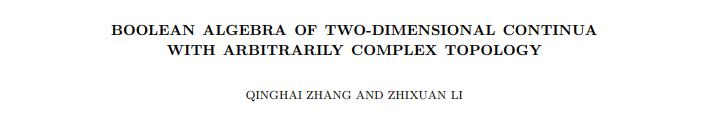
\includegraphics[width = \linewidth]{fig/articlename1.png}
        \item 2020年秋学期,在张老师的指导下,和学长合作完成项目微地震反问题.最终得到一个能根据
        检波器接收到的地震波信号输出合理的震源位置的程序.
        \item 2021年春学期,与学弟分工推进三维殷集的表示,及通过编程实现在计算机上计算
        三维殷集之间的布尔运算.
        \item 2021年秋学期,尝试使用matlab在张老师提出的CubicMars方法追踪动边界
        的过程中加入高精度追踪拓扑变化的时间点和发生位置.
    \end{enumerate}}
\end{frame}

\section{研究生项目详细介绍}
\subsection{微地震的反问题}

\begin{frame}[fragile]
    \frametitle{背景}
    \begin{itemize}
        \item  微地震通常是由于地质勘探或者一些开采活动导致地下裂缝错位,从而形成的
        低频率弹性波.
        \item 作为一种人为产生的地震, 其产生的信号经常出现于石油天然气工
        程作业. 近些年来, 国际上众多的研究机构与微震公司已经证明了
        微地震监测方法在油气田规划与开发方面的指导意义.
        \begin{columns}
            \column{0.4\linewidth}<1->
                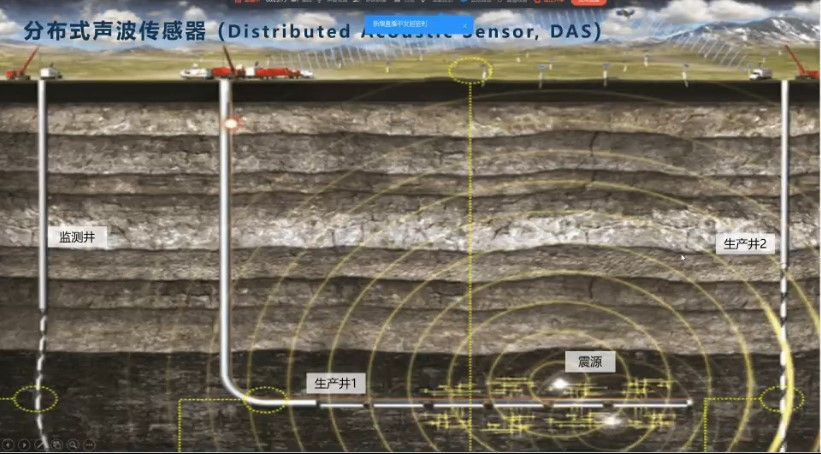
\includegraphics[width = \textwidth]{fig/s2p1.jpg}
            \column{0.6\linewidth}<1->
            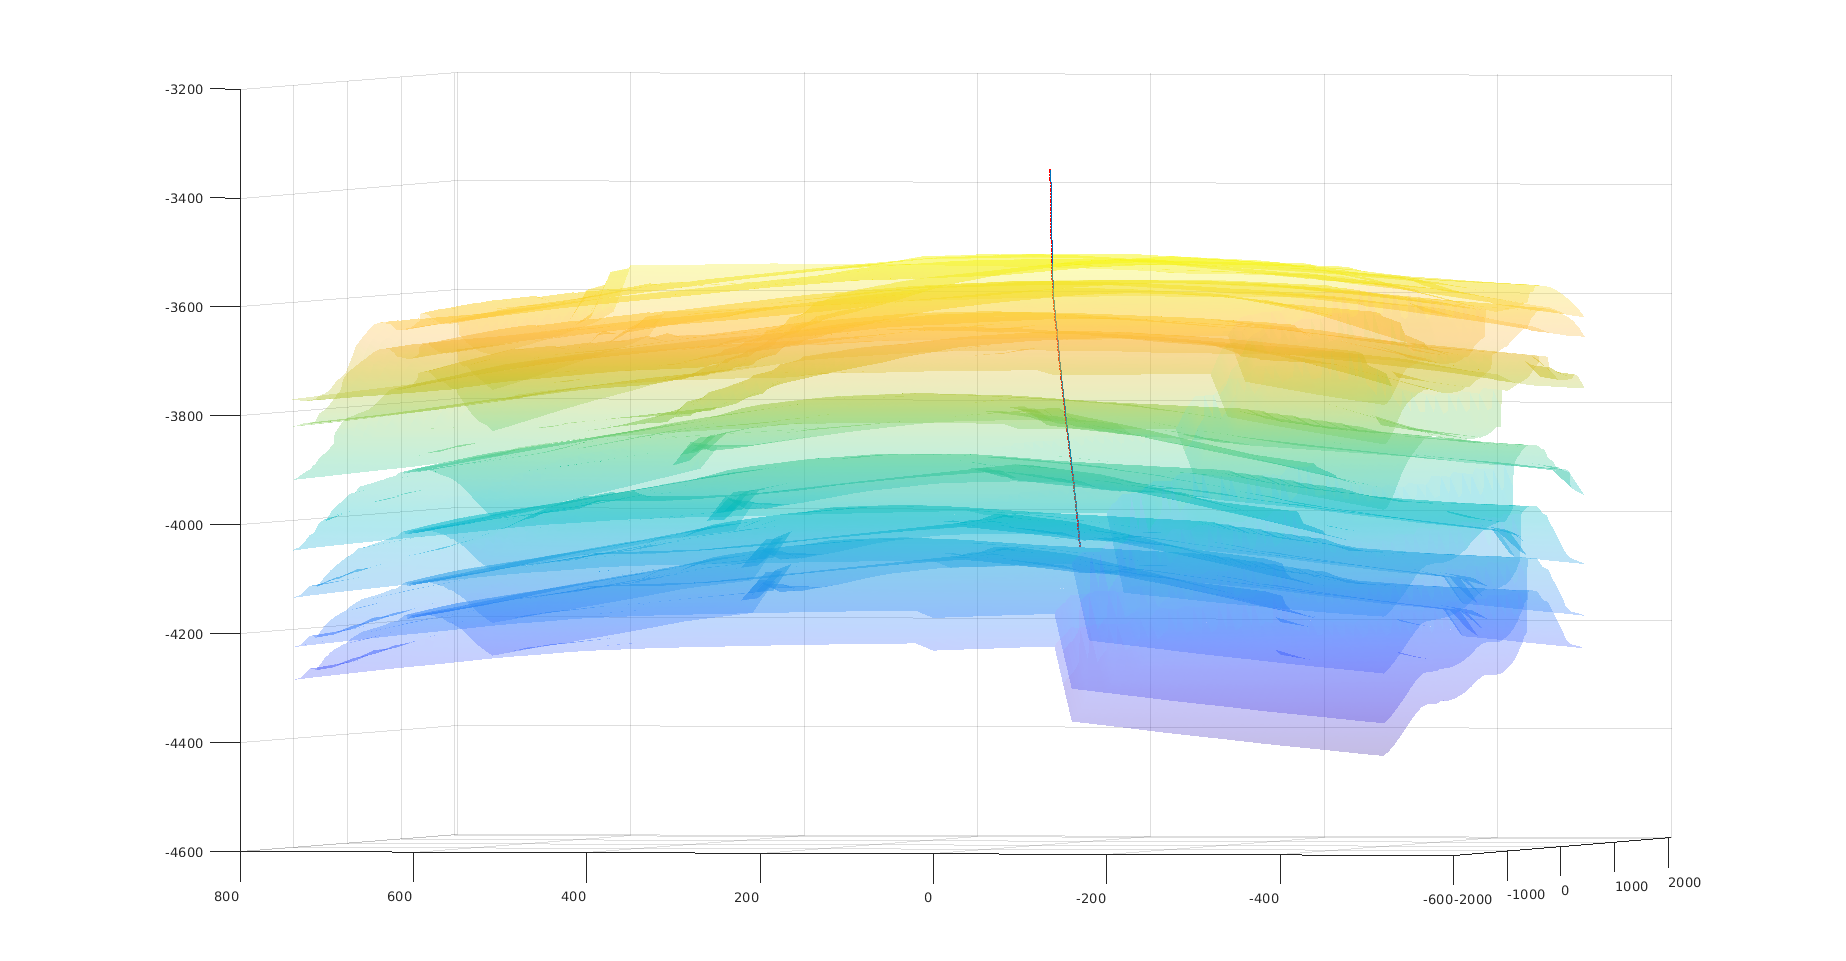
\includegraphics[width = \textwidth]{fig/layer.png}
        \end{columns}
        \item 因为地质结构的复杂,地震波非直线传播,并且微地震常发生于地下深处,检波器获取的信息少
        ,高精度反演非常困难. 
    \end{itemize}
\end{frame}

\begin{frame}
    \frametitle{解决思路}
    \begin{itemize}
        \item 因为检波器获取的到时是地震波最早到时,计算假设震源到检波器
        的时间,得到超定方程组.
        \begin{equation}
            V^lS^k - V^kS^l - V^lV^k(t^l-t^k) =0, \quad l \neq k.
        \end{equation}
        \item 采用多轮循环迭代的方式计算震源到检波器的时间.如下图二维示范
        \begin{columns}
            \column{0.5\linewidth}<1->
                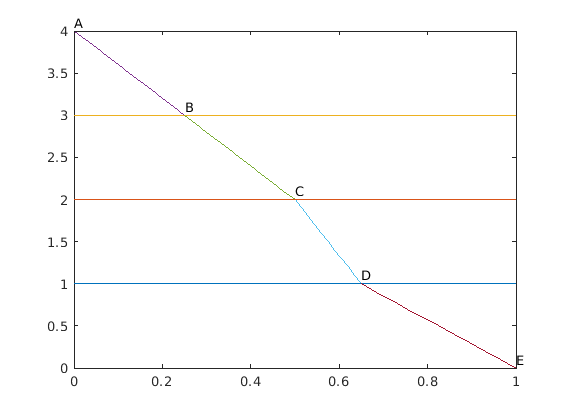
\includegraphics[width = \textwidth]{fig/layer1.png}
            \column{0.5\linewidth}<1->
            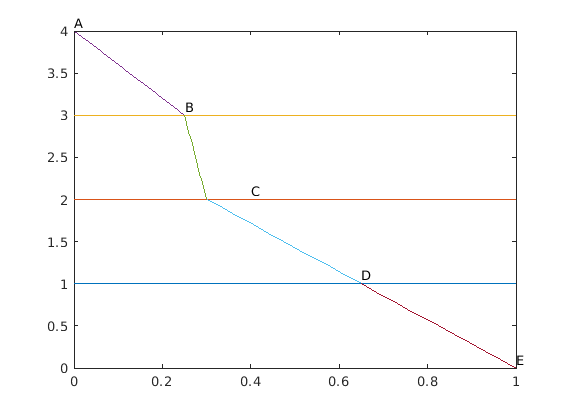
\includegraphics[width = \textwidth]{fig/layer2.png}
        \end{columns}
    \end{itemize}
\end{frame}

\begin{frame}
    \frametitle{妥协和学习}
    \begin{itemize}
        \item 计算时间的迭代可能因为地层复杂结构和断层的存在出现局部解.(加入模拟退火
        等随机因素)
        \item 震源位置的迭代会因为检波器过于集中在监测井这条线上导致无法
        正确得到xy坐标.(输出以监测井为轴心的圆)
    \end{itemize}
    当使用数学到工程实际中时,有时无法得到充分
    的已知条件从而不能给出准确的标准答案,需要及时的沟通改变双方的职责.
    \begin{center}
    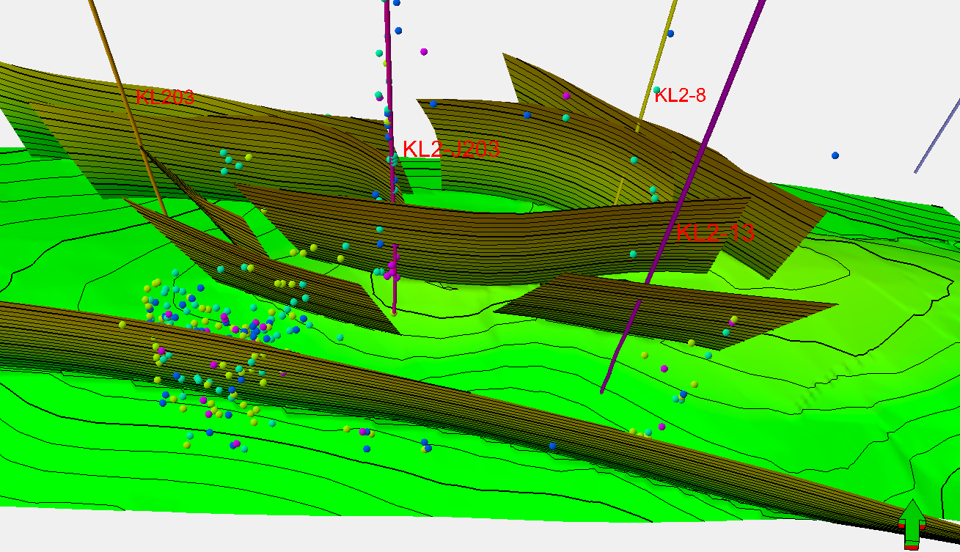
\includegraphics[width = 0.5\textwidth]{fig/sol122.png}
    \end{center}
\end{frame}

\subsection{三维殷集和布尔运算}
\begin{frame}
    \frametitle{研究背景}
    \begin{itemize}
        \item 流体建模相关研究少,数学模型和计算机算法都设计成避免在数值模拟时对流体
        进行几何建模.
        \begin{enumerate}
            \item VOF方法中使用各个单元的体积分数重建边界.
            \item FT方法追踪边界上的示踪点,按顺序连接得到边界.
            \item LS方法求解隐式函数得边界.
        \end{enumerate}
        这些方法舍弃了界面上的拓扑信息,几何问题转化为求解微分方程.过去几十年这些方法取得
        了大量的成果.
        \item 但是这些方法大部分只有二阶精度,二阶精度限制了曲率的估计,另一方面这些方法
        避免了几何建模使得很难严格地处理拓扑变化.
        \item 张老师2020年的论文中建立了一种流体建模的理论基础,在二维空间中
        提出了数学模型殷集来表示任意有物理意义的区域.
    \end{itemize}
\end{frame}

\begin{frame}
    \frametitle{二维殷集}
    \begin{itemize}
        \item 二维空间中,任一个殷集可以唯一表示为
        \[\mathcal{Y} = \cup_j^{\bot \bot}\cap_i \text{int}(\gamma_{j, i} ),\]
        Jordan Curve $\gamma_{j, i}$是$\mathcal{Y}$内第$j$个连通分量的第$i$条边.
        \item 高效实现了殷集上的布尔运算. 
        \begin{columns}
            \column{0.3\linewidth}<1->
                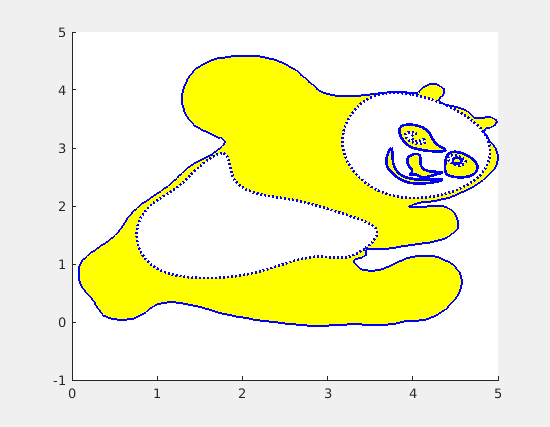
\includegraphics[width = \textwidth]{fig/p.png}
            \column{0.3\linewidth}<1->
            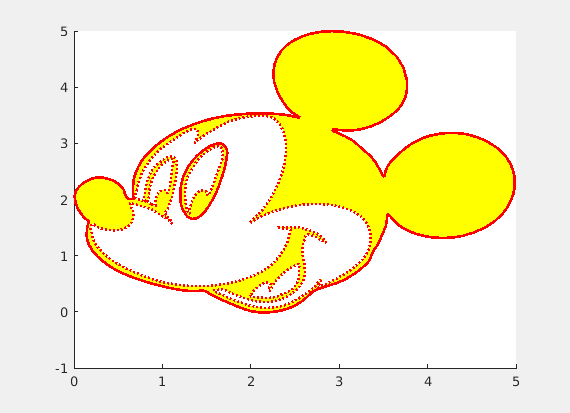
\includegraphics[width = \textwidth]{fig/m.png}
            \column{0.3\linewidth}<1->
            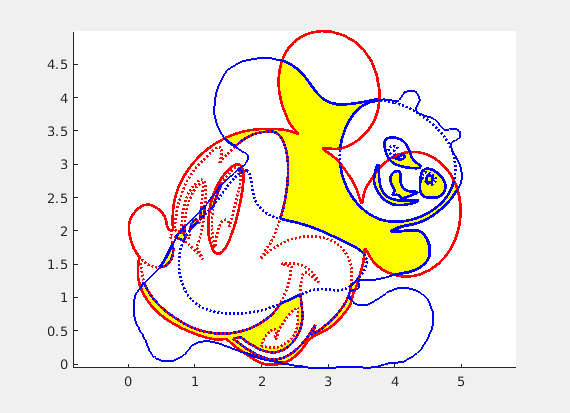
\includegraphics[width = \textwidth]{fig/pm.png}
        \end{columns}
    \end{itemize}
\end{frame}

\begin{frame}
    \frametitle{三维殷集的表示}
    \begin{itemize}
        \item 三维殷集:三维空间中边界有界的正则半解析开集.所有三维殷集构
        成的集合被称为殷空间,记为 $\mathbb{Y}$。
        \item 任一个殷集$\mathcal{Y} \in \mathbb{Y}$可以唯一表示为
        \[\mathcal{Y} = \cup_j^{\bot \bot} \cap_i \text{int}(\Gamma_{j, i}),\]
        黏合紧曲面$\Gamma_{j, i}$是$\mathcal{Y}$的第$j$个连通分量的第$i$个边界.
        \item 黏合紧曲面是与所有边界没有恰当交的闭合有向曲面.
    \end{itemize}
    \begin{columns}
        \column{0.5\linewidth}<1->
            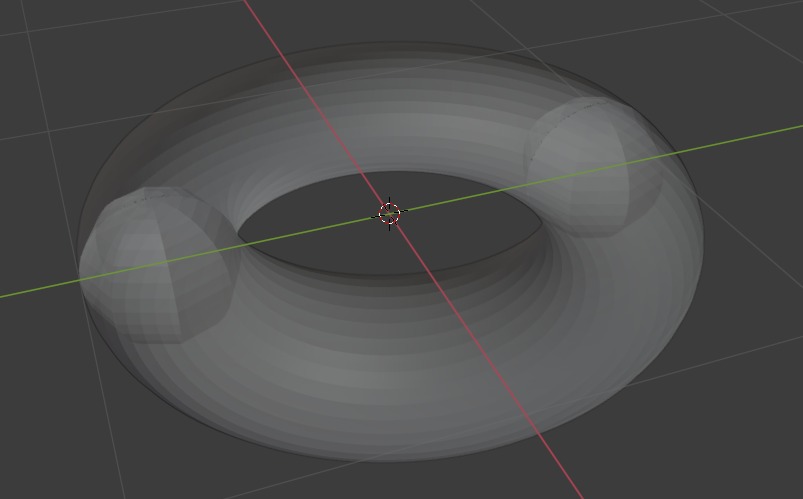
\includegraphics[width = \textwidth]{fig/s1.png}
        \column{0.5\linewidth}<1->
        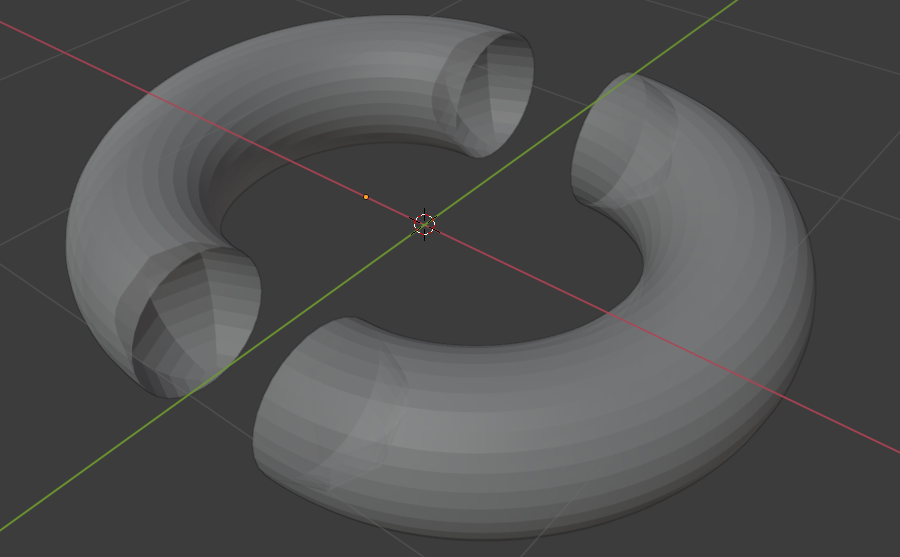
\includegraphics[width = \textwidth]{fig/s2.png}
    \end{columns}
\end{frame}

\begin{frame}
    \frametitle{布尔代数}
    \begin{itemize}
        \item 求布尔运算的两个殷集
        \begin{columns}
            \column{0.5\linewidth}<1->
                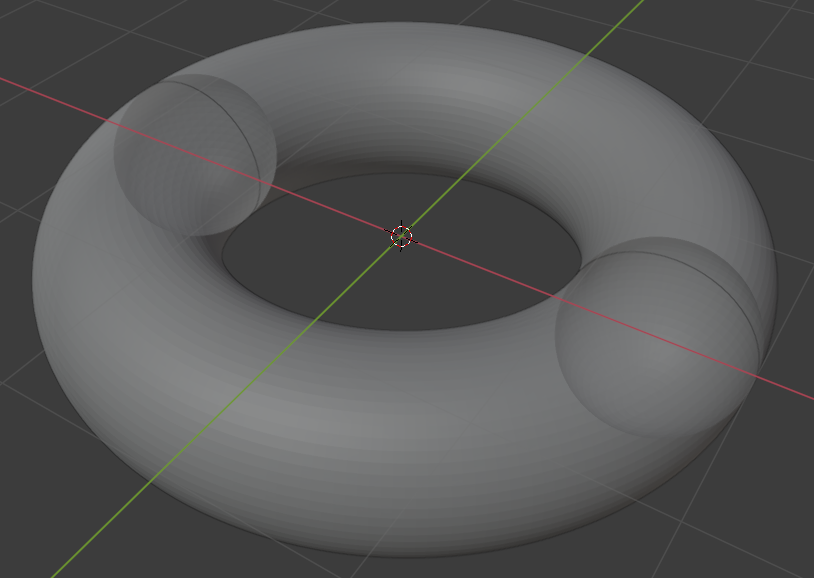
\includegraphics[width = \textwidth]{fig/s3.png}
            \column{0.5\linewidth}<1->
            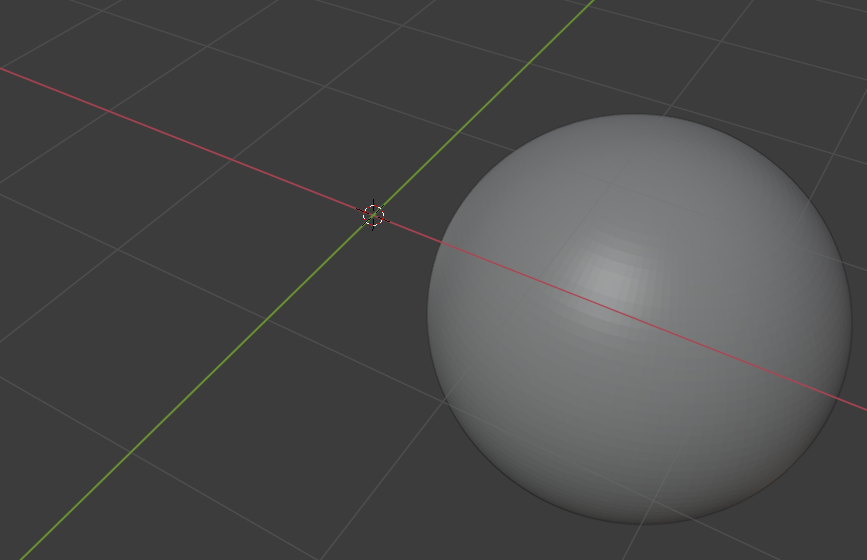
\includegraphics[width = \textwidth]{fig/s4.png}
        \end{columns}
        \item 交
        \begin{columns}
            \column{0.5\linewidth}<1->
                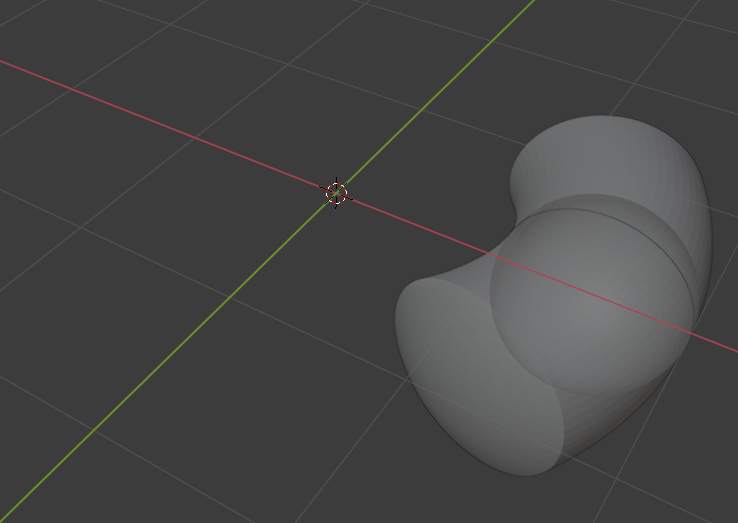
\includegraphics[width = \textwidth]{fig/s5.png}
            \column{0.5\linewidth}<1->
            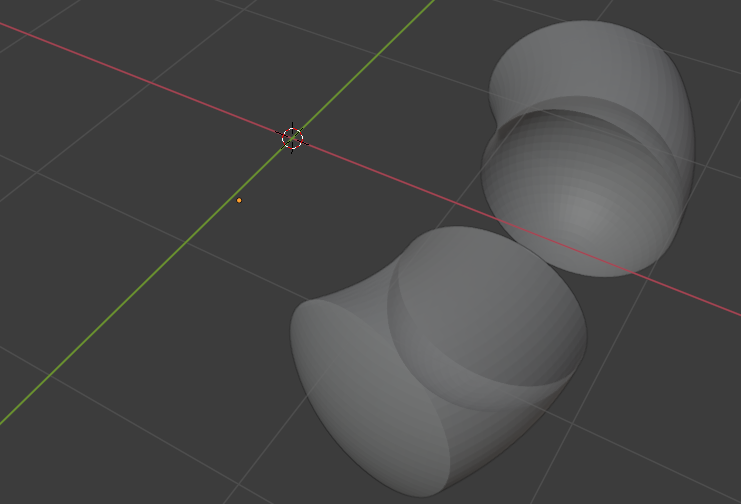
\includegraphics[width = \textwidth]{fig/s6.png}
        \end{columns}
    \end{itemize}
\end{frame}

\begin{frame}
    \begin{itemize}
        \item 并 \begin{columns}
            \column{0.5\linewidth}<1->
                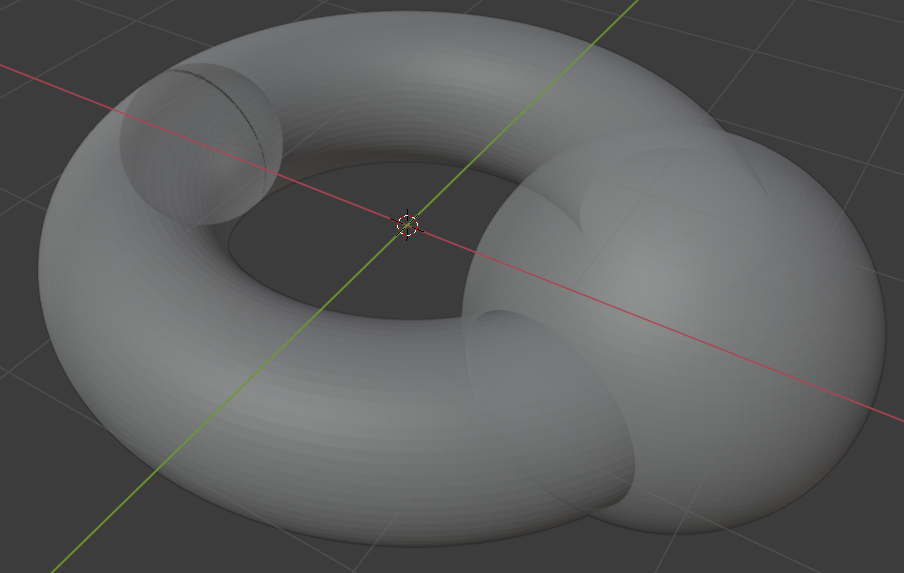
\includegraphics[width = \textwidth]{fig/s7.png}
            \column{0.5\linewidth}<1->
            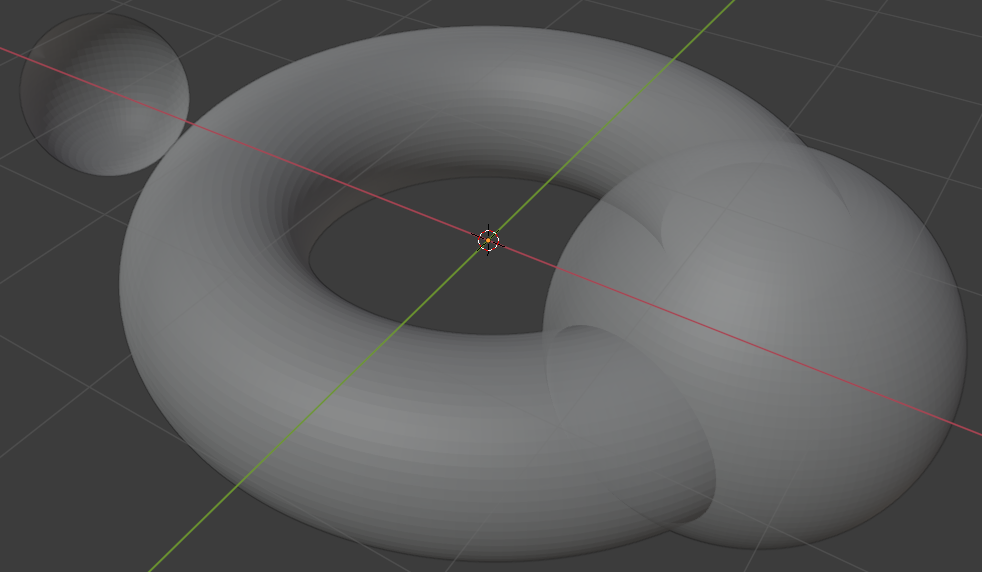
\includegraphics[width = \textwidth]{fig/s8.png}
        \end{columns}
        \item 复杂几何结构
        \begin{columns}
            \column{0.3\linewidth}<1->
                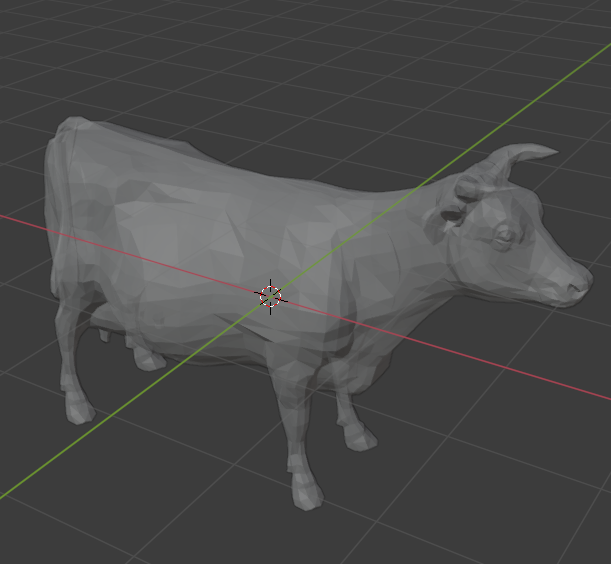
\includegraphics[width = \textwidth]{fig/s9.png}
            \column{0.3\linewidth}<1->
            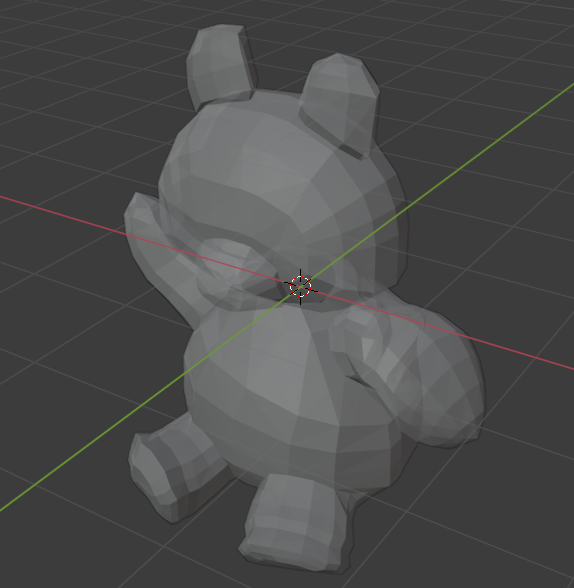
\includegraphics[width = \textwidth]{fig/s10.png}
            \column{0.3\linewidth}<1->
            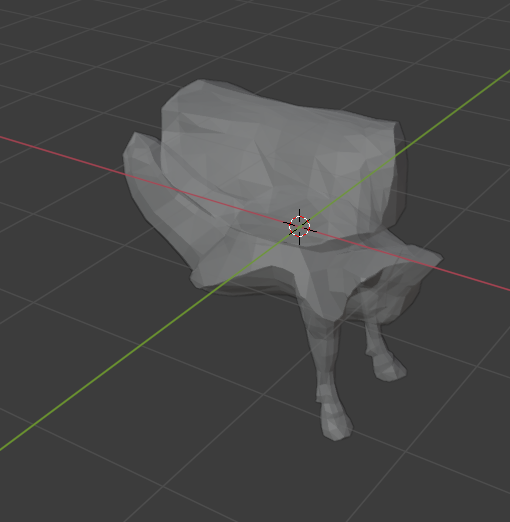
\includegraphics[width = \textwidth]{fig/s11.png}
        \end{columns}
    \end{itemize}
\end{frame}

\begin{frame}
    \frametitle{三维殷集建模的意义}
    \begin{itemize}
        \item 殷集对流体建模可以根据需要提高边界拟合精度.
        \item 殷集的表示方法可以同时保留边界上的非流形点,比如
        相切的边界.
        \item 通过殷集表示可以直接得到殷集闭包的Betti数$B_0, B_2$并期望可以得到
        $B_1$.
        \item 期望提供一套像实体建模一样的通用有效的流体建模理论体系,用于多相流研究。
    \end{itemize}
\end{frame}

\subsection{CubicMars方法追踪拓扑变化}
\begin{frame}
    \frametitle{研究背景}
    \begin{itemize}
        \item 多相流的研究在军事国防,医学仿生,核能工业,海洋工程,国民经济等许多重大
        领域中都占有举足轻重的地位; 而界面追踪问题是多相流数值计算中最基本的子问题之一.
        其重要性体现在
        \begin{enumerate}
            \item 界面追踪不可避免的影响到流相计算精度.
            \item 在表面张力不可忽略的多相流问题中,界面追踪准确性低会导致数值模拟
            结果脱离物理实际.
        \end{enumerate}
        \item 主流的VOF方法,FT方法,LS方法在过去都取得了巨大成功,但是随着多相流研究
        的进展,这些方法逐渐捉襟见肘.
        \item 张老师18年提出的CubicMars方法是一套普适理论用于对界面追踪问题的分析,
        是时空一致四阶以上精度的界面追踪方法.
    \end{itemize}
    
\end{frame}

\begin{frame}
    \frametitle{工作的方向} 
    \begin{itemize}
        \item 在CubicMars方法的基础上,结合二维殷集,增添对拓扑变化的处理.
        \item 需要在有拓扑变化的流相追踪过程中保持计算精度.
        \item 期望同样能高精度捕捉流相拓扑变化的时间点和位置.
    \end{itemize}
\end{frame}

\section{博士阶段的研究计划}
\begin{frame}
    \frametitle{海洋内波的理论,模型与计算}
    \begin{itemize}
        \item 潜艇湍流尾迹的海洋表面特征等内波现象的研究, 用于潜艇追踪和隐身.
        (军科委基础加强重点项目).
        \begin{figure}
            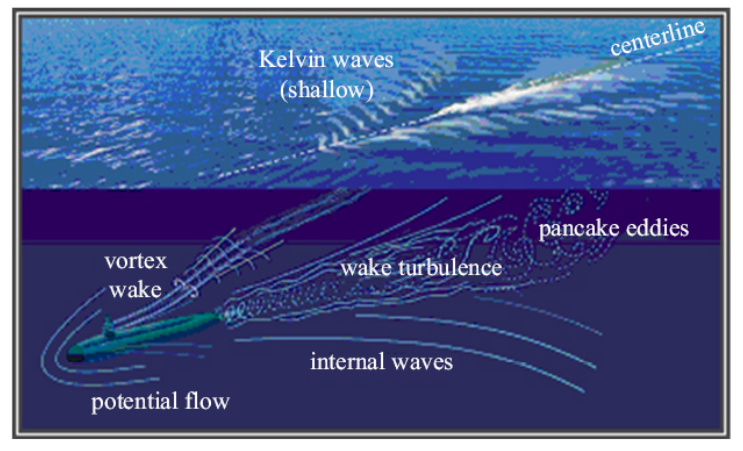
\includegraphics[width = 0.7\textwidth]{fig/s12.png};
            \caption{水下潜艇产生的各种尾迹示意图, 包括开尔文尾迹, 内波, 湍流尾迹, 涡尾迹, 煎
            饼旋涡.}
        \end{figure}
    \end{itemize}
\end{frame}

\section*{}
\begin{frame}
    \centering\huge
    \textcolor{red}{请各位老师批评指针!}
\end{frame}
% \end{CJK}
\end{document}